\documentclass{beamer}
\usetheme{Dresden}

\title{Socratic Models: Composing Zero-Shot Multimodal Reasoning with Language}
\author{Andy Zeng, Maria Attarian, Brian Ichter, et al.}
\date{\today}

\begin{document}

\frame{\titlepage}

\begin{frame}{Introduction}
    This paper proposes Socratic Models (SMs), a framework that leverages diverse pretrained models, allowing them to communicate and jointly perform tasks without additional training, thereby enhancing multimodal reasoning capabilities.
\end{frame}

\begin{frame}{Methods}
    SMs employ a modular approach where pretrained models exchange information via language-based prompts, enabling various applications like image captioning and video understanding without the need for fine-tuning.
\end{frame}

\begin{frame}{Results}
    The evaluation demonstrates that SMs achieve competitive performance on various benchmarks, setting new zero-shot state-of-the-art results in tasks such as image captioning and video-to-text retrieval while enabling innovative applications in egocentric perception and assistive dialogue.
\end{frame}

\begin{frame}{Discussion}
    SMs highlight the potential of integrating heterogeneous models to capture multimodal functionalities more efficiently without requiring extensive domain-specific data or finetuning, although there are inherent limitations regarding model reliability and biases.
\end{frame}

\begin{frame}{Conclusion}
    Socratic Models represent a promising approach for enhancing multimodal capabilities in AI systems while emphasizing the importance of responsible application and monitoring for unintended use.
\end{frame}

\begin{frame}{Extracted Figure}
    \centering
    \begin{figure}
        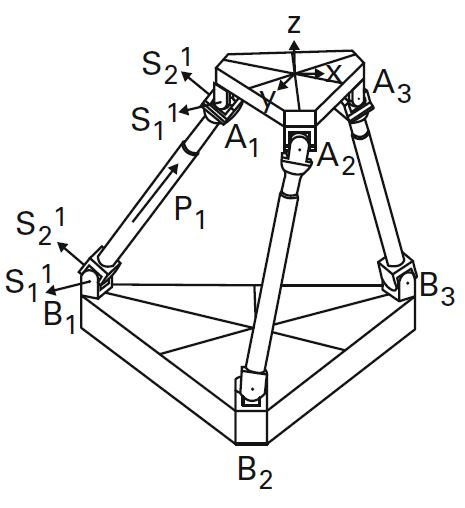
\includegraphics[width=0.8\textwidth]{extracted_images/figure_2_1.png}  % Relative path inside slides/
    \end{figure}
\end{frame}

\begin{frame}{Extracted Figure}
    \centering
    \begin{figure}
        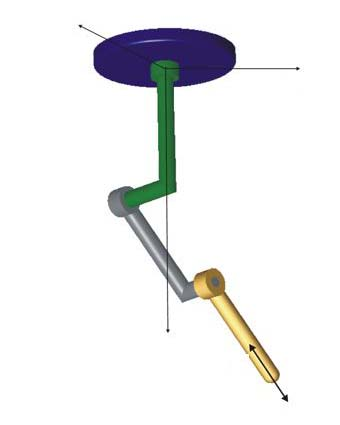
\includegraphics[width=0.8\textwidth]{extracted_images/figure_4_1.png}  % Relative path inside slides/
    \end{figure}
\end{frame}

\begin{frame}{Extracted Figure}
    \centering
    \begin{figure}
        \includegraphics[width=0.8\textwidth]{extracted_images/figure_4_2.png}  % Relative path inside slides/
    \end{figure}
\end{frame}

\begin{frame}{Extracted Figure}
    \centering
    \begin{figure}
        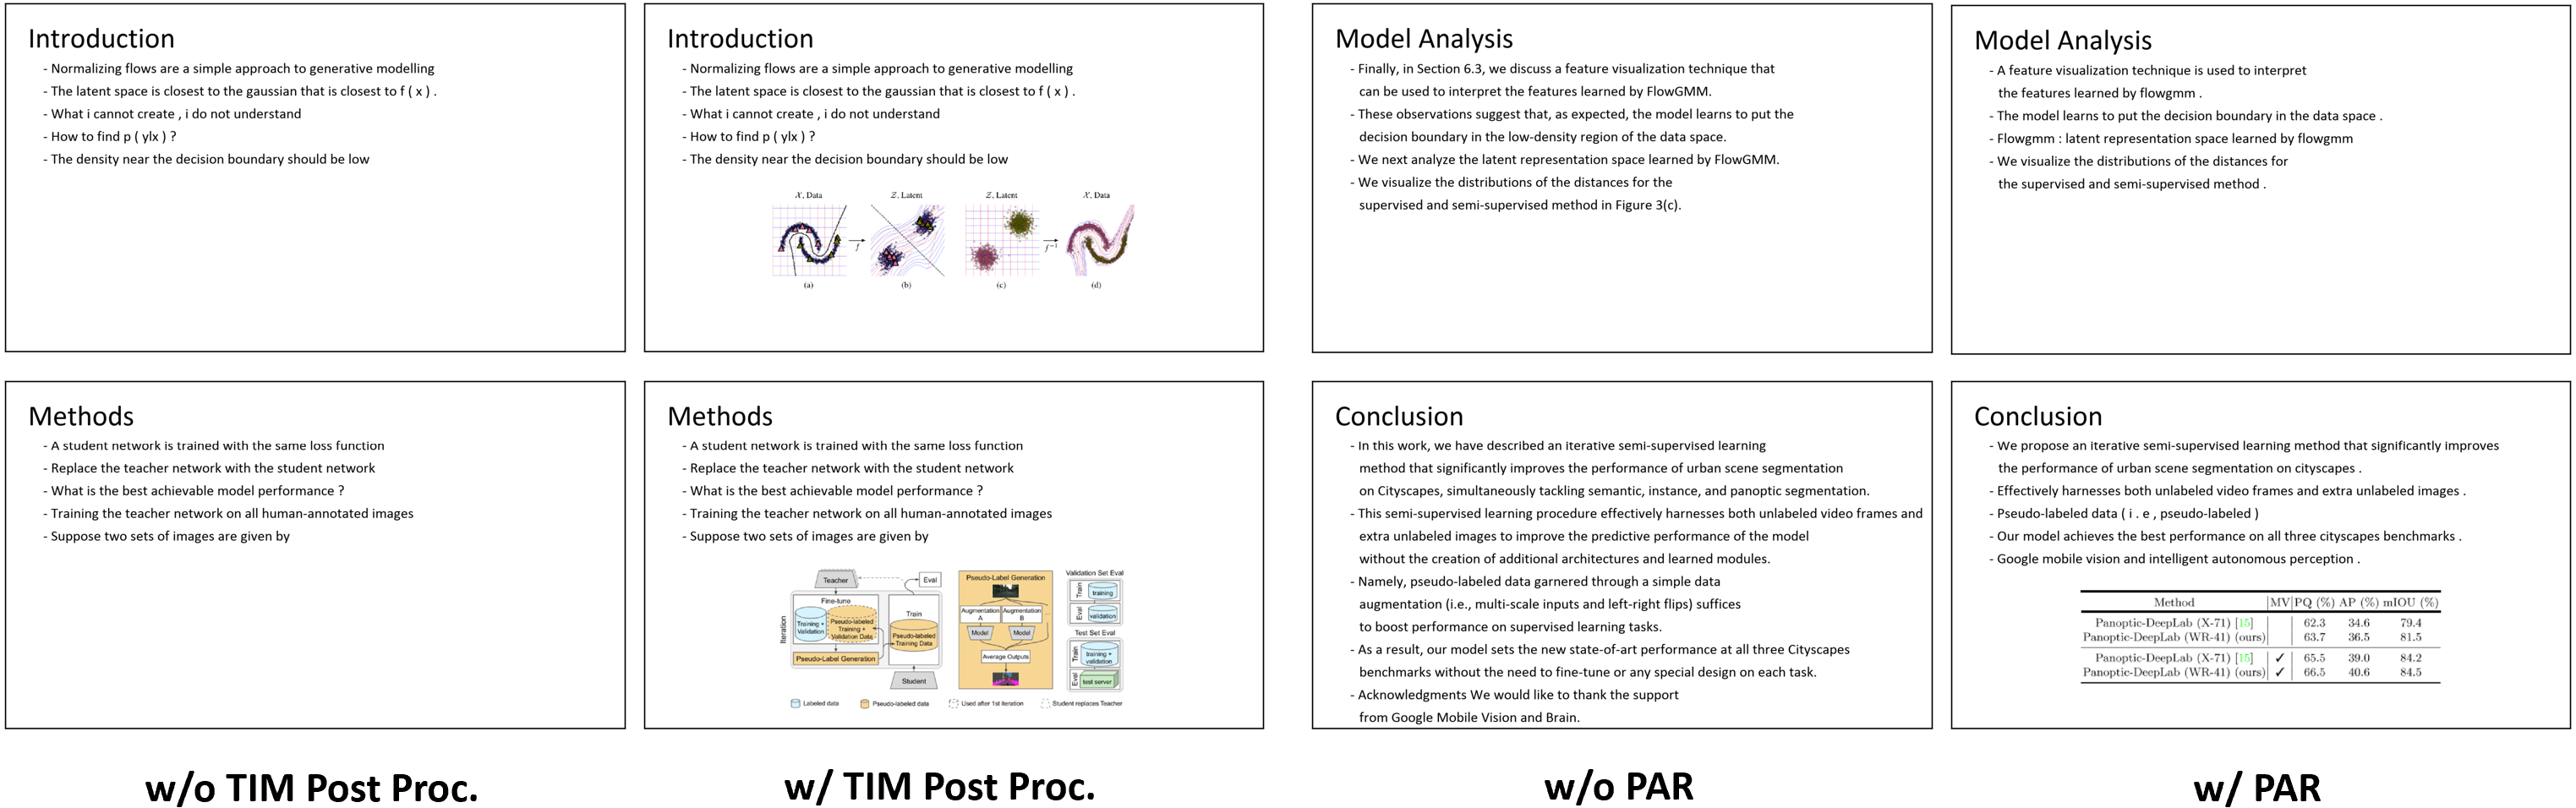
\includegraphics[width=0.8\textwidth]{extracted_images/figure_7_1.png}  % Relative path inside slides/
    \end{figure}
\end{frame}

\begin{frame}{Extracted Figure}
    \centering
    \begin{figure}
        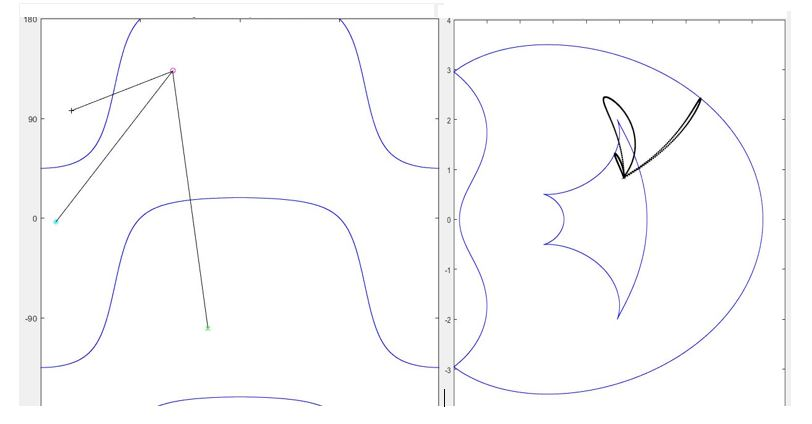
\includegraphics[width=0.8\textwidth]{extracted_images/figure_8_1.png}  % Relative path inside slides/
    \end{figure}
\end{frame}

\begin{frame}{Extracted Figure}
    \centering
    \begin{figure}
        \includegraphics[width=0.8\textwidth]{extracted_images/figure_9_1.png}  % Relative path inside slides/
    \end{figure}
\end{frame}

\begin{frame}{Extracted Figure}
    \centering
    \begin{figure}
        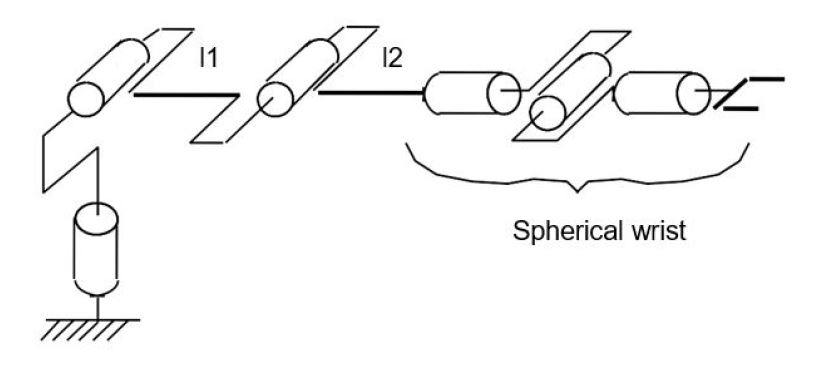
\includegraphics[width=0.8\textwidth]{extracted_images/figure_19_1.png}  % Relative path inside slides/
    \end{figure}
\end{frame}

\begin{frame}{Extracted Figure}
    \centering
    \begin{figure}
        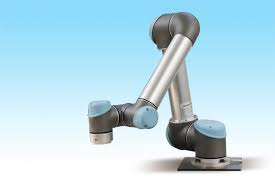
\includegraphics[width=0.8\textwidth]{extracted_images/figure_20_1.png}  % Relative path inside slides/
    \end{figure}
\end{frame}

\begin{frame}{Extracted Figure}
    \centering
    \begin{figure}
        \includegraphics[width=0.8\textwidth]{extracted_images/figure_21_1.png}  % Relative path inside slides/
    \end{figure}
\end{frame}

\begin{frame}{Extracted Figure}
    \centering
    \begin{figure}
        \includegraphics[width=0.8\textwidth]{extracted_images/figure_22_1.png}  % Relative path inside slides/
    \end{figure}
\end{frame}

\begin{frame}{Extracted Figure}
    \centering
    \begin{figure}
        
\includegraphics[width=0.8\textwidth]{extracted_images/figure_24_1.png}  % Relative path inside slides/
    \end{figure}
\end{frame}

\begin{frame}{Extracted Figure}
    \centering
    \begin{figure}
        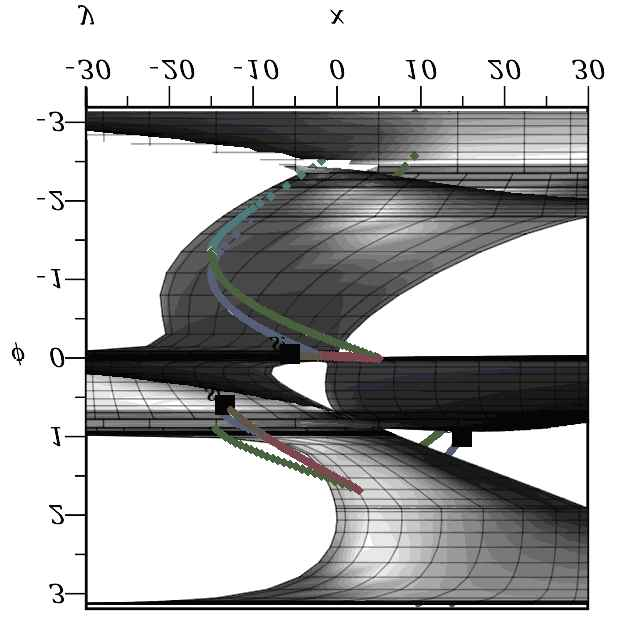
\includegraphics[width=0.8\textwidth]{extracted_images/figure_26_1.png}  % Relative path inside slides/
    \end{figure}
\end{frame}

\begin{frame}{Extracted Figure}
    \centering
    \begin{figure}
        \includegraphics[width=0.8\textwidth]{extracted_images/figure_28_1.png}  % Relative path inside slides/
    \end{figure}
\end{frame}

\begin{frame}{Extracted Figure}
    \centering
    \begin{figure}
        
\includegraphics[width=0.8\textwidth]{extracted_images/figure_29_1.png}  % Relative path inside slides/
    \end{figure}
\end{frame}

\end{document}